%\documentclass[aps,prb,twocolumn,groupedaddress,nofootinbib,floatfix]{revtex4}
\documentclass{article}
\usepackage{mathtools}
\usepackage{mathrsfs}
\usepackage[parfill]{parskip}

\usepackage[margin=1in]{geometry}

\begin{document}

\title{EM PE Implementation and Usage}

%
\author{Ben Champion}

\date{\today}

\maketitle

\section{Models}

\subsection{Simple analytic kilonova model}

\textbf{Note:} some of this text comes directly from \cite{Villar_2017}.

The single-component, two-component, and three-component analytic kilonova models provided with the code are an implementation of the model described in \cite{Villar_2017}.
In the following equations, $M$ is the $r$-process ejecta mass and $v$ is the ejecta velocity.
Note that for now we assume the ejecta consists entirely of $r$-process material, so $M$ is the full ejecta mass.
The radioactive heating rate at time $t$ is given by \cite{Korobkin_2012}:
\begin{equation}
    L_\text{in}(t) = 4 \times 10^{18} M \times \left [ 0.5 - \pi^{-1} \arctan \left ( \frac {t - t_0} {\sigma} \right ) \right ]^{1.3} \text{ erg s}^{-1}
\end{equation}
where $t_0 = 1.3$ s and $\sigma = 0.11$ s are constants.

Only a fraction of $L_\text{in}$ powers the kilonova, given by the thermalization efficiency $\epsilon_\text{th}$.
This is approximated analytically in \cite{Barnes_2016}:
\begin{equation}
    \epsilon_\text{th}(t) = 0.36 \left [ e^{-a t} + \frac {\ln(1 + 2 b t^d)} {2 b t^d} \right ]
\end{equation}
The parameters $a$, $b$, and $d$ are constants that depend on the ejecta mass and velocity; an interpolation of Table 1 in \cite{Barnes_2016} is used in the model.

The bolometric luminosity is calculated as
\footnote{\cite{Villar_2017} is missing a factor of time in the denominator (this can be seen from the units -- our $L_\text{bol}$ has the correct units of erg s$^{-1}$). 
The factor of 1/$t_d$ seems to produce reasonable results with the correct units, and better aligns with e.g. \cite{Chatzopoulos_2012}.}
\begin{equation}
    L_\text{bol}(t) = \frac {2} {t_d} \exp{\left ( \frac {-t^2} {t_d^2} \right ) }
                    \int_0^t L_\text{in} \epsilon_\text{th} \exp{\left ( \frac {t^2} {t_d^2} \right ) } \frac {t} {t_d} dt
\end{equation}
where $t_d$ is the diffusion timescale, $t_d = \sqrt{2 \kappa M / \beta v c}$, $\kappa$ is the opacity, and $\beta = 13.7$ is a dimensionless constant related to the ejecta's geometry.

Lightcurves are calculated by assuming the kilonova behaves as a blackbody photosphere that expands at a velocity $v$.
The blackbody temperature is generally defined by its bolometric luminosity; however, once it cools to a critical temperature $T_c$, the photosphere recedes into the ejecta and the temperature remains fixed.
The photosphere temperature is
\footnote{\cite{Villar_2017} has a mistake here: $\sigma_\text{SB}$ should not be squared.}
\begin{equation} \label{T_c}
    T_\text{phot}(t) = \max \left [ \left ( \frac {L_\text{bol}(t)} {4 \pi \sigma_\text{SB} v^2 t^2} \right )^{1/4}, T_c \right]
\end{equation}

When $T_\text{phot} > T_c$, the photosphere radius is simply $R_\text{phot} = v t$.
When $T_\text{phot} = T_c$ (i.e. the photosphere has receded into the ejecta), the photosphere radius is
\begin{equation}
    R_\text{phot}(t) = \left ( \frac {L_\text{bol}(t)} {4 \pi \sigma_\text{SB} T_c^4} \right )^{1/2}
\end{equation}

The flux density at frequency $\nu$ is given in \cite{Metzger_2017}:
\begin{equation}
    F_\nu(t) = \frac {2 \pi h \nu^3} {c^2} \frac {1} {\exp{(h \nu / k T_\text{photo}(t))} - 1} \frac {R_\text{photo}^2(t)} {D^2}
\end{equation}
where $D$ is the source distance.
We use a fixed fiducial distance of $D = 10$ pc to calculate $F_\nu(t)$, then calculate AB magnitude with a distance modulus if necessary.

For the single-component model $\kappa$ and $T_c$ are free parameters.
For the two-component and three-component variations $\kappa$ takes a fixed value for each component and $T_c$ can either be fit to the data or fixed to any value specified by the user.
To compute multi-component lightcurves we assume each component has a photosphere that evolves independently of the others.
The total flux density is the sum of the flux densities of the individual components.

\section{Parameter Estimation}

\subsection{Likelihood Function}

For lightcurve magnitude $x(t)$, model value $m(t; \theta)$ computed with parameters $\theta$, and errors $\delta x(t)$ and $\delta m(t)$, the log-likelihood is
\begin{equation}
    \ln \mathcal{L}(\theta) = -0.5 \sum \frac {(x(t) - m(t; \theta))^2} {\delta x(t)^2 + \delta m(t; \theta)^2}
\end{equation}
where the sum is taken over every data point in every band used in the analysis.

This log-likelihood is implemented as a method in \texttt{EM\_PE}'s \texttt{sampler} class, which can be imported and used in other codes.
The joint gravitational wave and EM log-likelihood is the sum of the individual log-likelihoods.

\subsection{Injection/Recovery Example}

A simple parameter estimation test using fake data can be run after installing the \texttt{EM\_PE} code to ensure it functions properly.
The repository contains a \texttt{Makefile} that generates reproducable parameter estimation runs.
To run the injection/recovery test:
\begin{verbatim}
$ make test_kilonova_3c
$ cd pe_runs/test_kilonova_3c/
$ ./sample.sh
\end{verbatim}
This series of commands will generate a posterior sample file, \texttt{samples.txt}.
Note that the default settings assume the code is being run on a machine with many CPU cores available, so it computes the likelihood in 8 parallel processes.
It will run without issue on a less powerful computer, but \texttt{sample.sh} should be modified to use fewer cores (e.g. set \texttt{--nprocs 2} to use two cores).

To produce a corner plot and lightcurve plot, run
\begin{verbatim}
$ ./plot_corner.sh
$ ./plot_lc.sh
\end{verbatim}
This will produce plots similar to Figure \ref{fig:corner} and Figure \ref{fig:lightcurves}.

\begin{figure}[!ht]
    \centering
    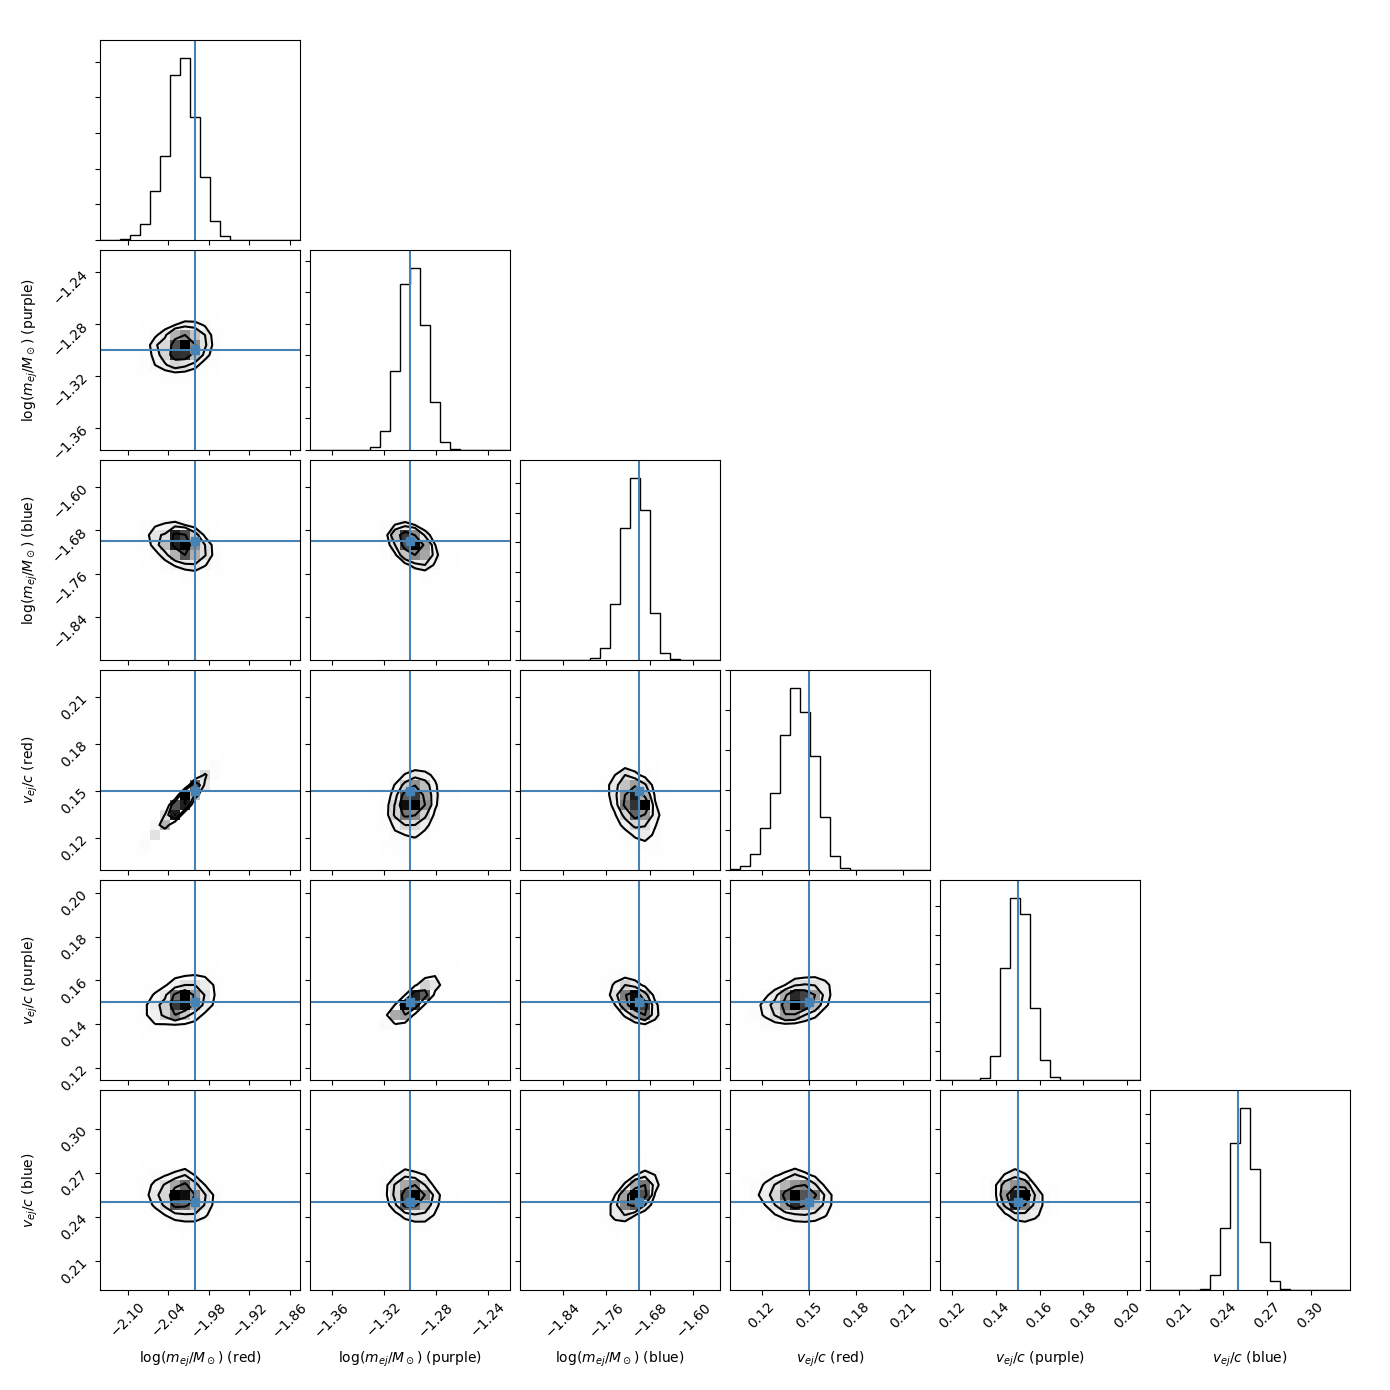
\includegraphics[width=6.5in]{corner.png}
    \caption{Posterior distribution for the injection/recovery test (the blue lines show the true parameter values). For this example, $T_c$ was fixed for each component and the distance was fixed to 40.0 Mpc.}
    \label{fig:corner}
\end{figure}

\begin{figure}[!ht]
    \centering
    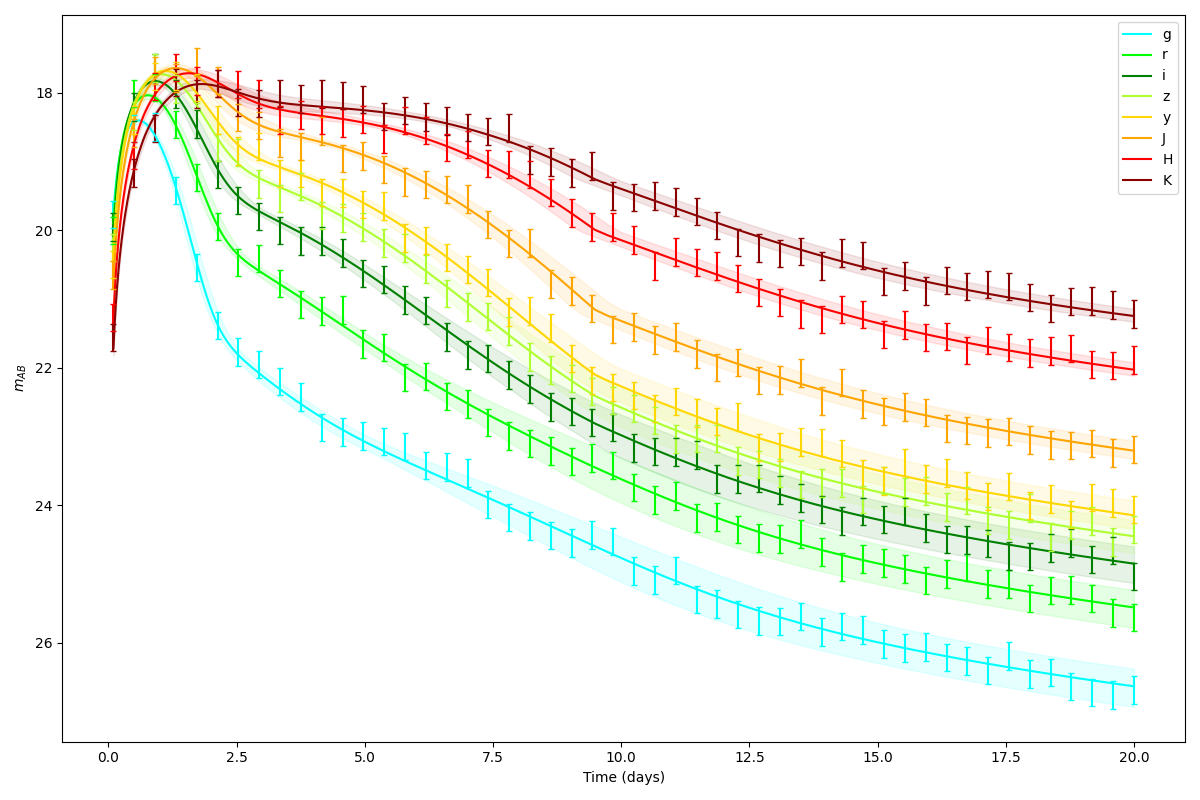
\includegraphics[width=6.5in]{lc.png}
    \caption{Fake photometry data and lightcurve models for the injection/recovery test. The solid line shows the lightcurve model evaluated at the maximum-likelihood parameters.}
    \label{fig:lightcurves}
\end{figure}

\subsection{GW170817 Example Analysis}

\textit{Coming soon}

\clearpage

\bibliographystyle{h-physrev5.bst}
\bibliography{bibliography}

\end{document}
